\documentclass[a4paper,utf8]{article}
\usepackage[heading,fancyhdr]{ctex}
\usepackage{amsmath,amssymb,geometry,lastpage,ulem}
\usepackage{array,tabularx,tabulary,mhchem,xspace}
\usepackage{floatrow,subfig,multirow,bigstrut}
\usepackage{siunitx,booktabs,longtable,graphicx,xfrac,nameref}
\lineskiplimit=1pt
\lineskip=3pt
\geometry{
    top=25.4mm, 
    left=25mm, 
    right=25mm, 
    bottom=25mm,
    headsep=5.9mm,
}
\ctexset{
    section = {format+=\raggedright}
}
\newcommand{\fgref}[1]{图~\ref{#1}\xspace}
\newcommand{\seqref}[1]{式~(\ref{#1})}
\newcommand{\expinfo}[7][无]{
    {\zihao{-3}\bfseries\songti
    实验名称:\uline{\hfill\mbox{#2}\hfill} \\[2.9mm]
    学\quad 号:\uline{\makebox[25mm]{#3}}\hfill
    姓\quad 名:\uline{\makebox[25mm]{#4}}\hfill
    班\quad 级:\uline{\makebox[25mm]{#5}} \\[2.9mm]
    合作者:\uline{\makebox[25mm]{#1}} \hfill
    桌\quad 号:\uline{\makebox[25mm]{#6}}\hfill\makebox[25mm+4em]{}\\[2.9mm]
    实验日期:\uline{\makebox[30mm]{#7}}\hfill\mbox{} \\[58.7mm]
    }
}
\newcommand{\pointingbox}{
    {\zihao{4}\bfseries\songti%
    实验考核\\[3mm]
    \extrarowheight=3mm
    \begin{tabularx}{150mm}{|X|X|X|X|X|}\hline
        \hfil 项目 \hfil  & \hfil 实验预习 \hfil & \hfil 实验过程 \hfil & \hfil 分析与讨论 \hfil & \hfil 总评 \hfil \\[3mm] \hline
        \hfil 评价 \hfil &  &  &  &  \\[3mm] \hline
    \end{tabularx}
    }
}
\newcommand{\derivative}[2]{\frac{\mathrm{d} #1}{\mathrm{d} #2}}
\newcommand{\thinking}[2]{\textbf{#1}\\
答:\begin{minipage}[t]{0.85\textwidth}
    #2
\end{minipage}}
\pagestyle{fancy}
\fancyhf{} \fancyhead[C]{电路基础实验} \fancyfoot[C]{\thepage~/~\pageref{LastPage}}
\newcounter{Rownumber}
\newcommand*{\Rown}{\stepcounter{Rownumber}\theRownumber}
\newcommand*{\resetRown}{\setcounter{Rownumber}{0}}
\newcommand{\qrange}[3]{\qtyrange[range-phrase = \text{$\sim$},range-units =single]{#1}{#2}{#3}}
\floatsetup[table]{capposition=top}
\newcolumntype{C}{>{\hfil}X<{\hfil}}
\renewcommand{\Nameref}[1]{\textbf{\ref{#1}~\nameref{#1}}} %导入导言
\ExecuteOptions{draft}
\begin{document}
\begin{center}
    {\mbox{}\\[7em]\zihao{2}\bfseries\songti%
    电路基础实验报告}\\[34mm]
    \expinfo[王慷]{二阶电路动态过程的研究}{22301056}{王俊杰}{22 材物}{27}{2024.6.11}
\end{center}
\newpage

\section{实验目的}
\begin{enumerate}
    \item 研究二阶电路动态过程的零状态响应和零输入响应的基本规律和特点。
    \item 分析电路参数 R、L、C 对二阶电路动态过程响应的影响。
    \item 学习使用双线示波器观察动态过程波形的方法。
    \item 学习方波信号源的使用方法。
\end{enumerate}

\section{实验原理}%简单描述,含必要的公式和附图;
二阶线性电路。从电路原理我们知道,用二阶线性常微分方程来描述的电路称为二阶线性电路。本实验研究有一个电感和电阻,又有一个电容的二阶电路,在方波激励时响应的动态过程。\par
对于 RLC 串联的二阶电路,无论是零状态响应,还是零输入响应,电路过渡过程中性质完全由特征方程上 $LC_P^2+RC_P+1=0$ 的特征根 $P_1$,$P_2$来决定。
$$P_{1,2}=-\frac{R}{2L}\pm\sqrt{(\frac{R}{2L})^2-(\frac{1}{\sqrt{LC}})^2}=-\delta\pm\sqrt{\delta^2-\omega_0^2}$$
从上式可看出,特征根 $P_1$,$P_2$ 实际由电路 R、L、C 三个元件参数的数值大小来决定:如果 $R>2\sqrt{L/C}$,电路动态过程的性质为过阻尼的非振荡的过程;如果 $R=2\sqrt{L/C}$,电路动态过程的性质为临界阻尼过程;如果 $R<2\sqrt{L/C}$,电路动态过程的性质为欠阻尼的衰减振荡;如果 $R=0$,电路动态过程为等幅振荡;如果 $R<0$,电路动态过程为增幅振荡;\par
从上述可知,通过改变电路的参数电阻 R(含负阻)、电感 L 或电容 C 的值,均可使电路发生上述几种不同性质的过渡过程。为研究二阶电路动态过程的性质,实际单元板上电路参数 R、L、C 各给出 $2 \sim 3$ 个值。\par

\section{实验仪表}
    实验电路见电路原理实验箱《二阶电路动态过程的研究》单元,$R_w=0 \sim 1\unit{\kilo\ohm}$、$R2= 10\unit{\ohm}$、$C1= 0.1\unit{\uF}$、$C2= 0.22\unit{\uF}$、$C3= 0.047\unit{\uF}$、$L1= 5\unit{\mH}$、$L2= 10\unit{\mH}$。

\section{实验内容与结果}
    \subsection{测试准备}
    \subsection{RLC 电路动态过程的测试与观察}
\clearpage
\section{实验结果}
    \subsection{欠阻尼}
    电路参数:$L= \SI{5}{\mH}$,$C= \SI{0.1}{\uF}$,$R=\SI{100}{\ohm}$
    \begin{figure}[!ht]
        \includegraphics[width=0.71\textwidth]{1q.pdf}
        \caption{欠阻尼理论图像}
    \end{figure}
    \begin{figure}[!ht]
        \subfloat[$U_\text{s}$]{\includegraphics[width=0.35\textwidth]{1sq.jpg}}\hspace{6mm}
        \subfloat[$U_\text{C}$]{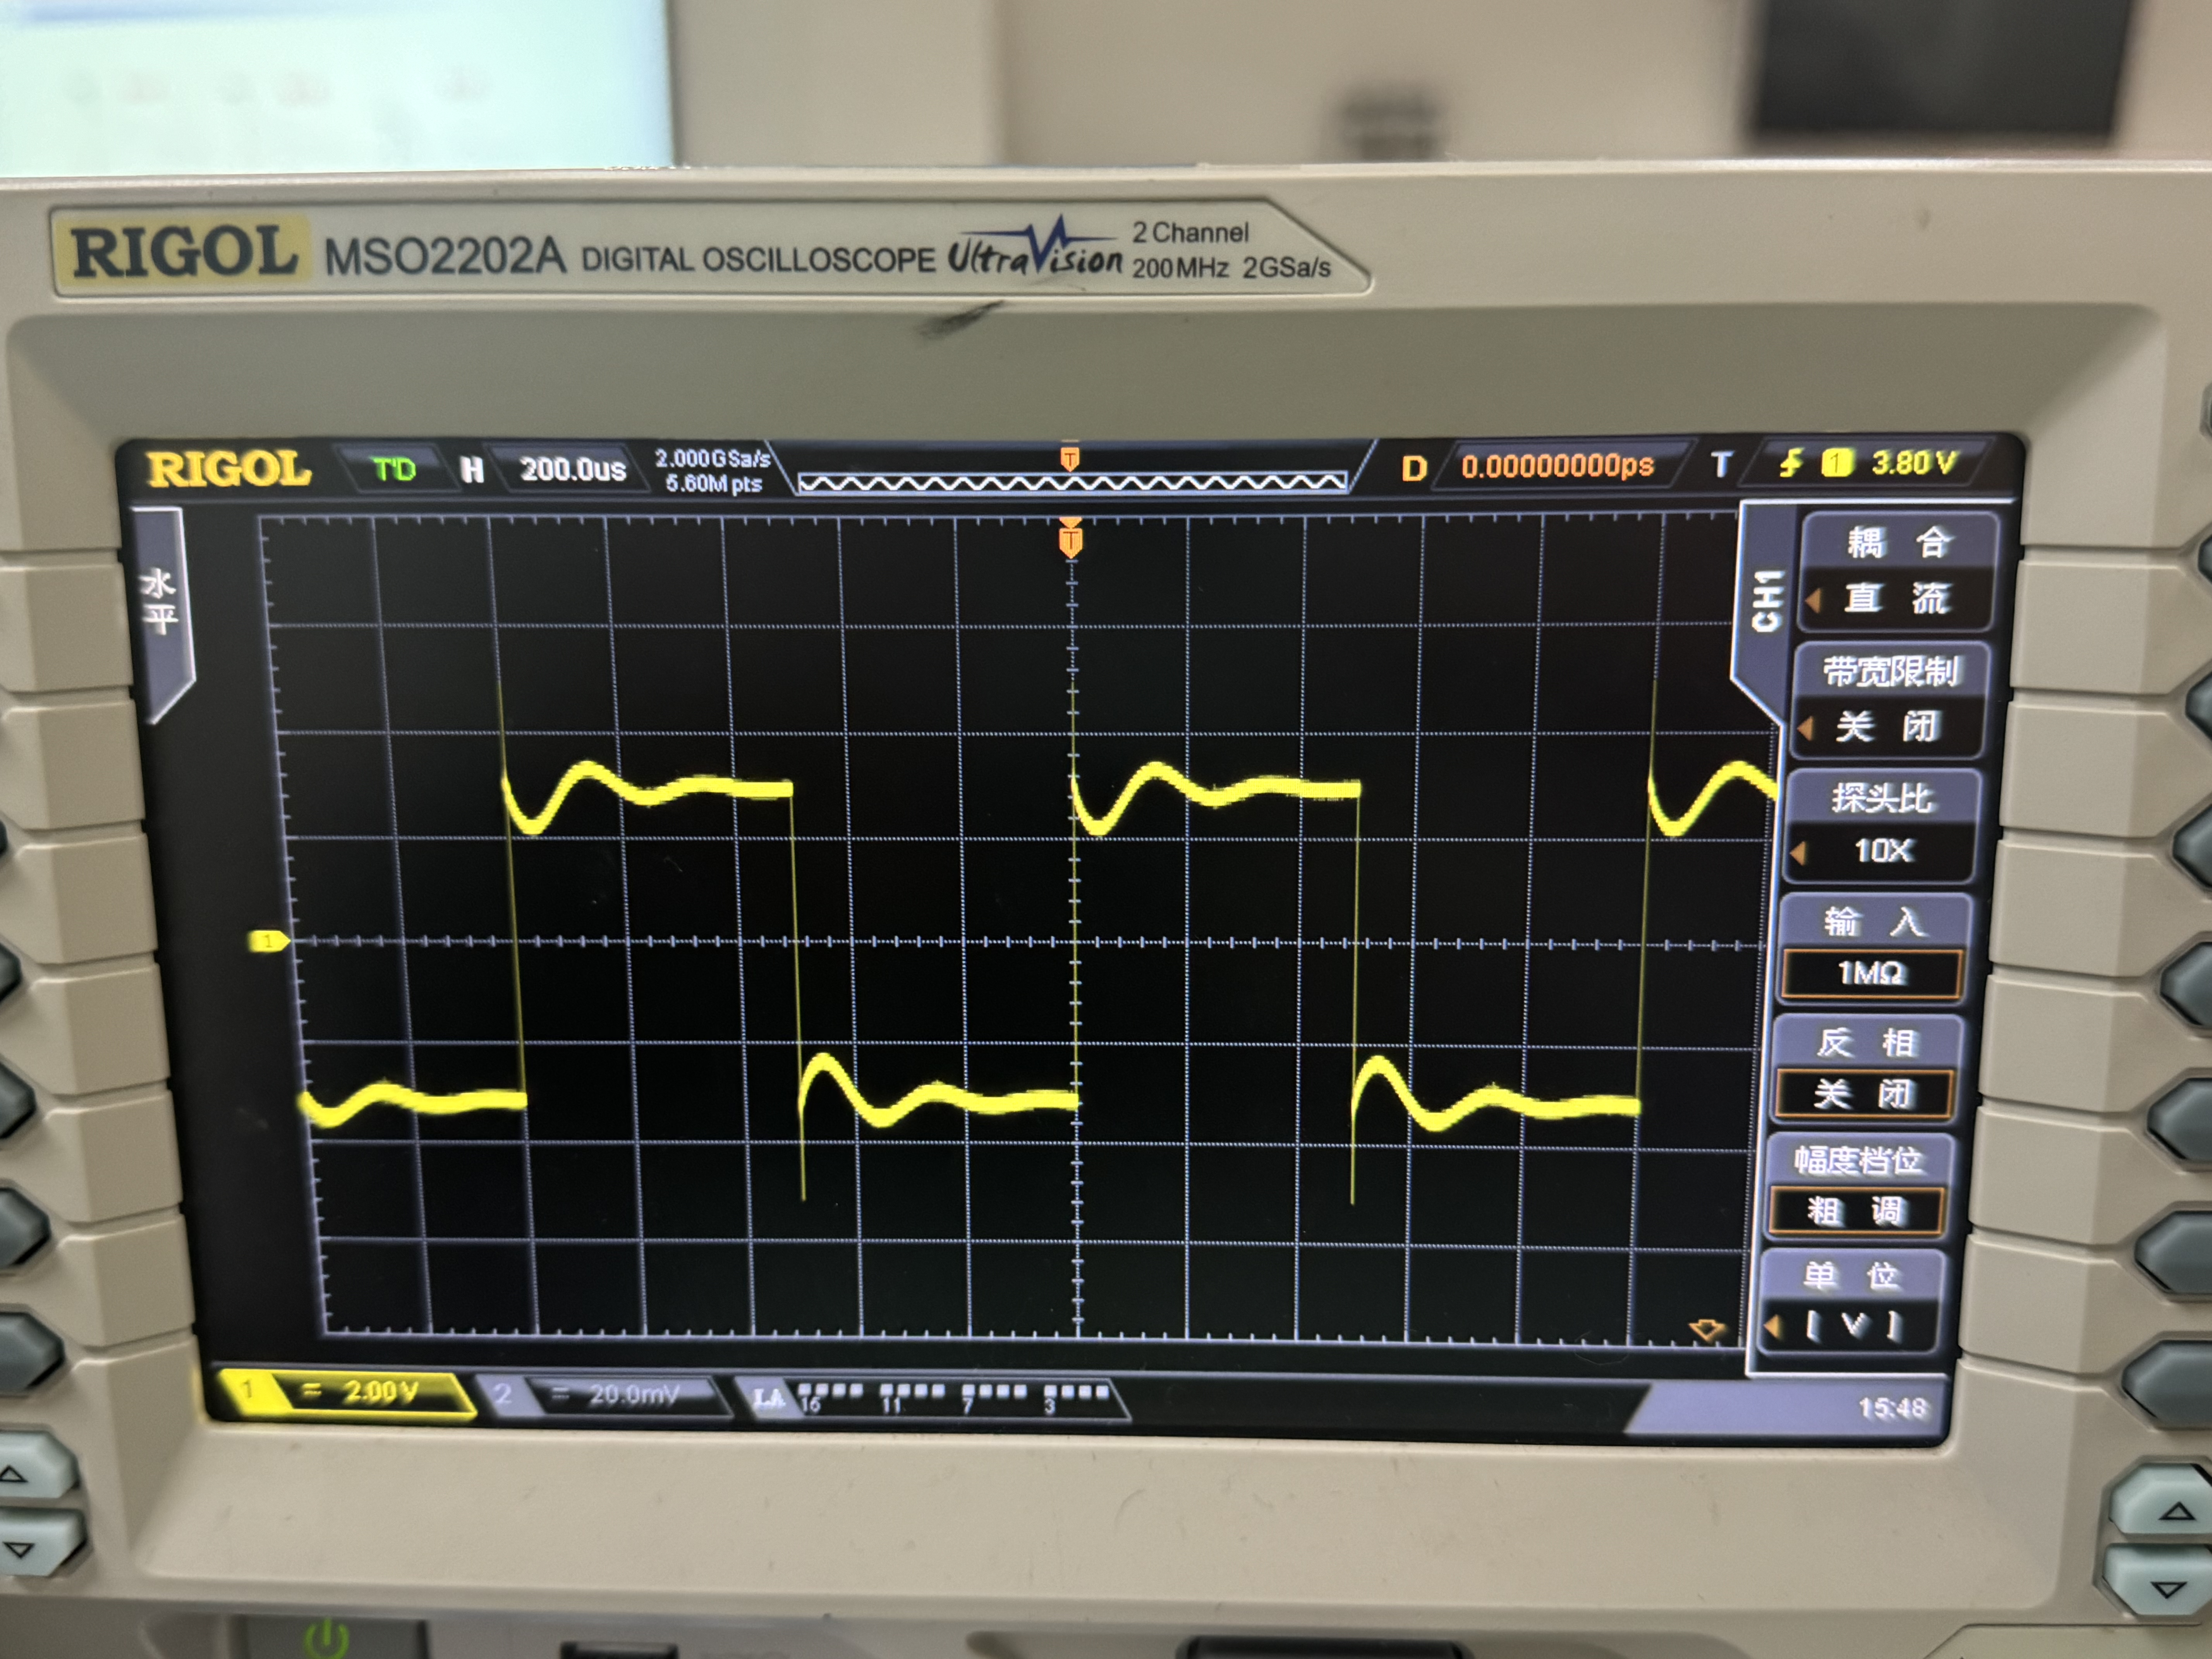
\includegraphics[width=0.35\textwidth]{1Cq.jpg}}\\
        \subfloat[$U_\text{L}$]{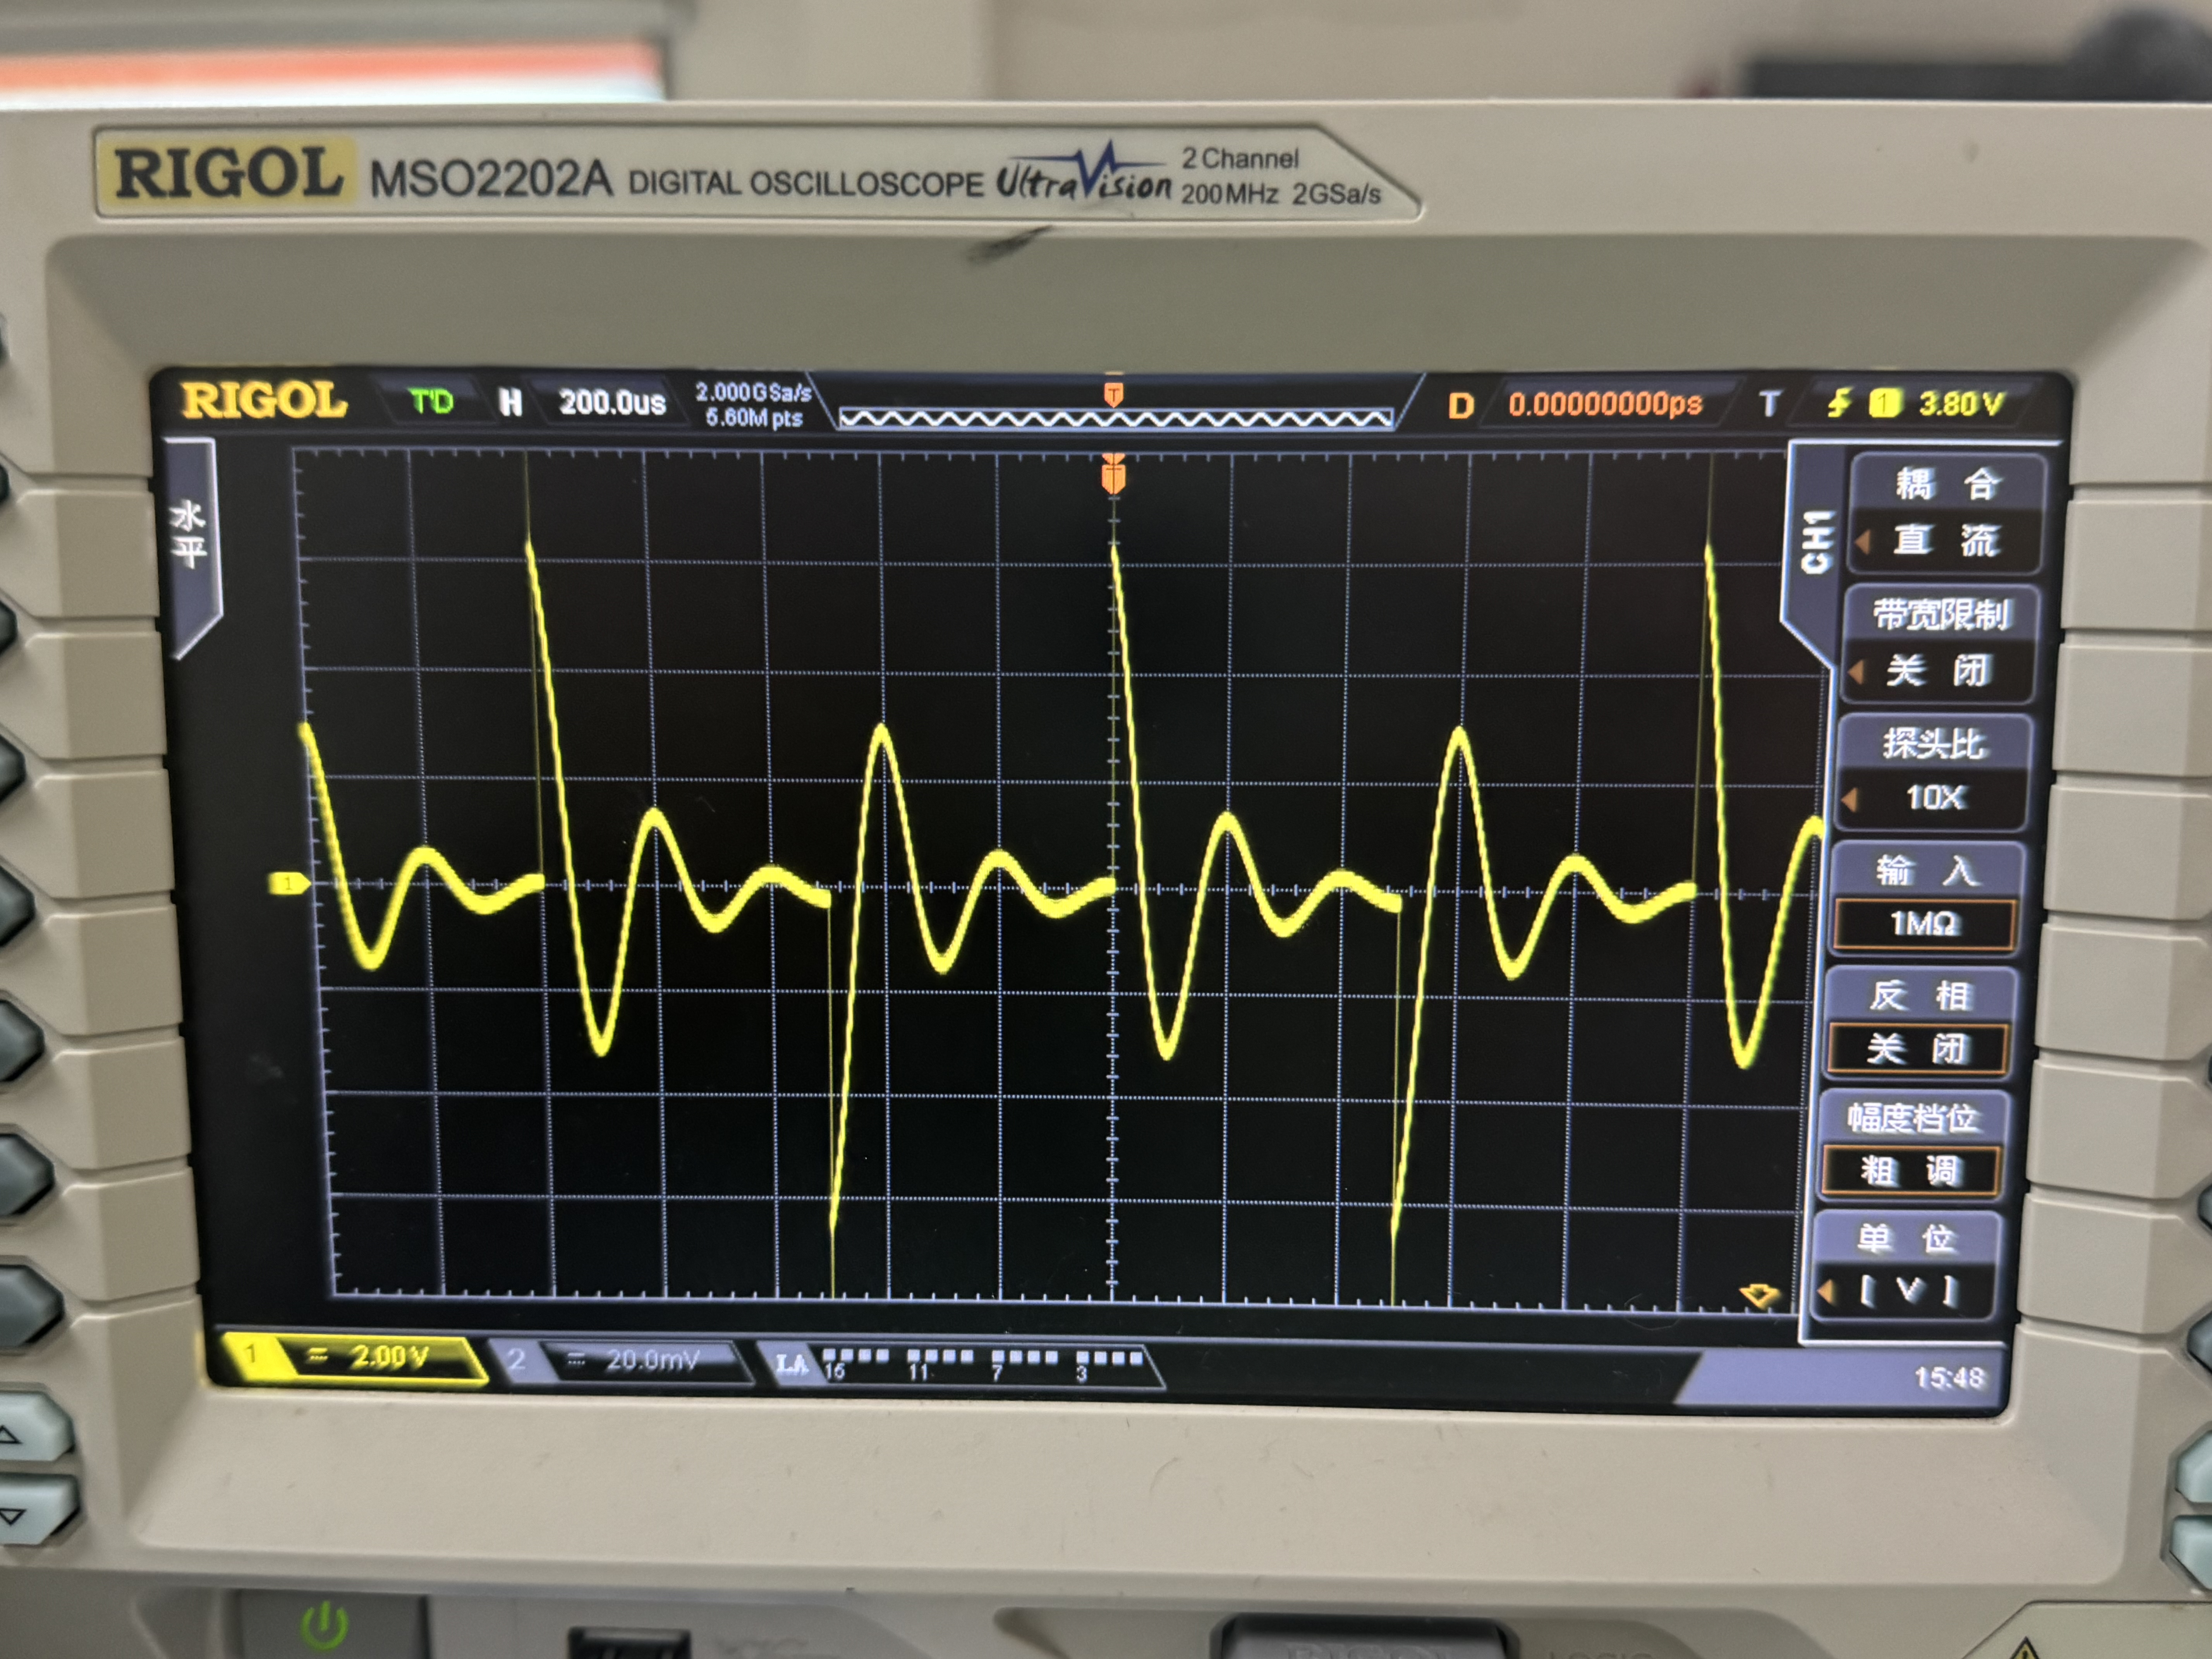
\includegraphics[width=0.35\textwidth]{1Lq.jpg}}\hspace{6mm}
        \subfloat[$U_\text{R}$]{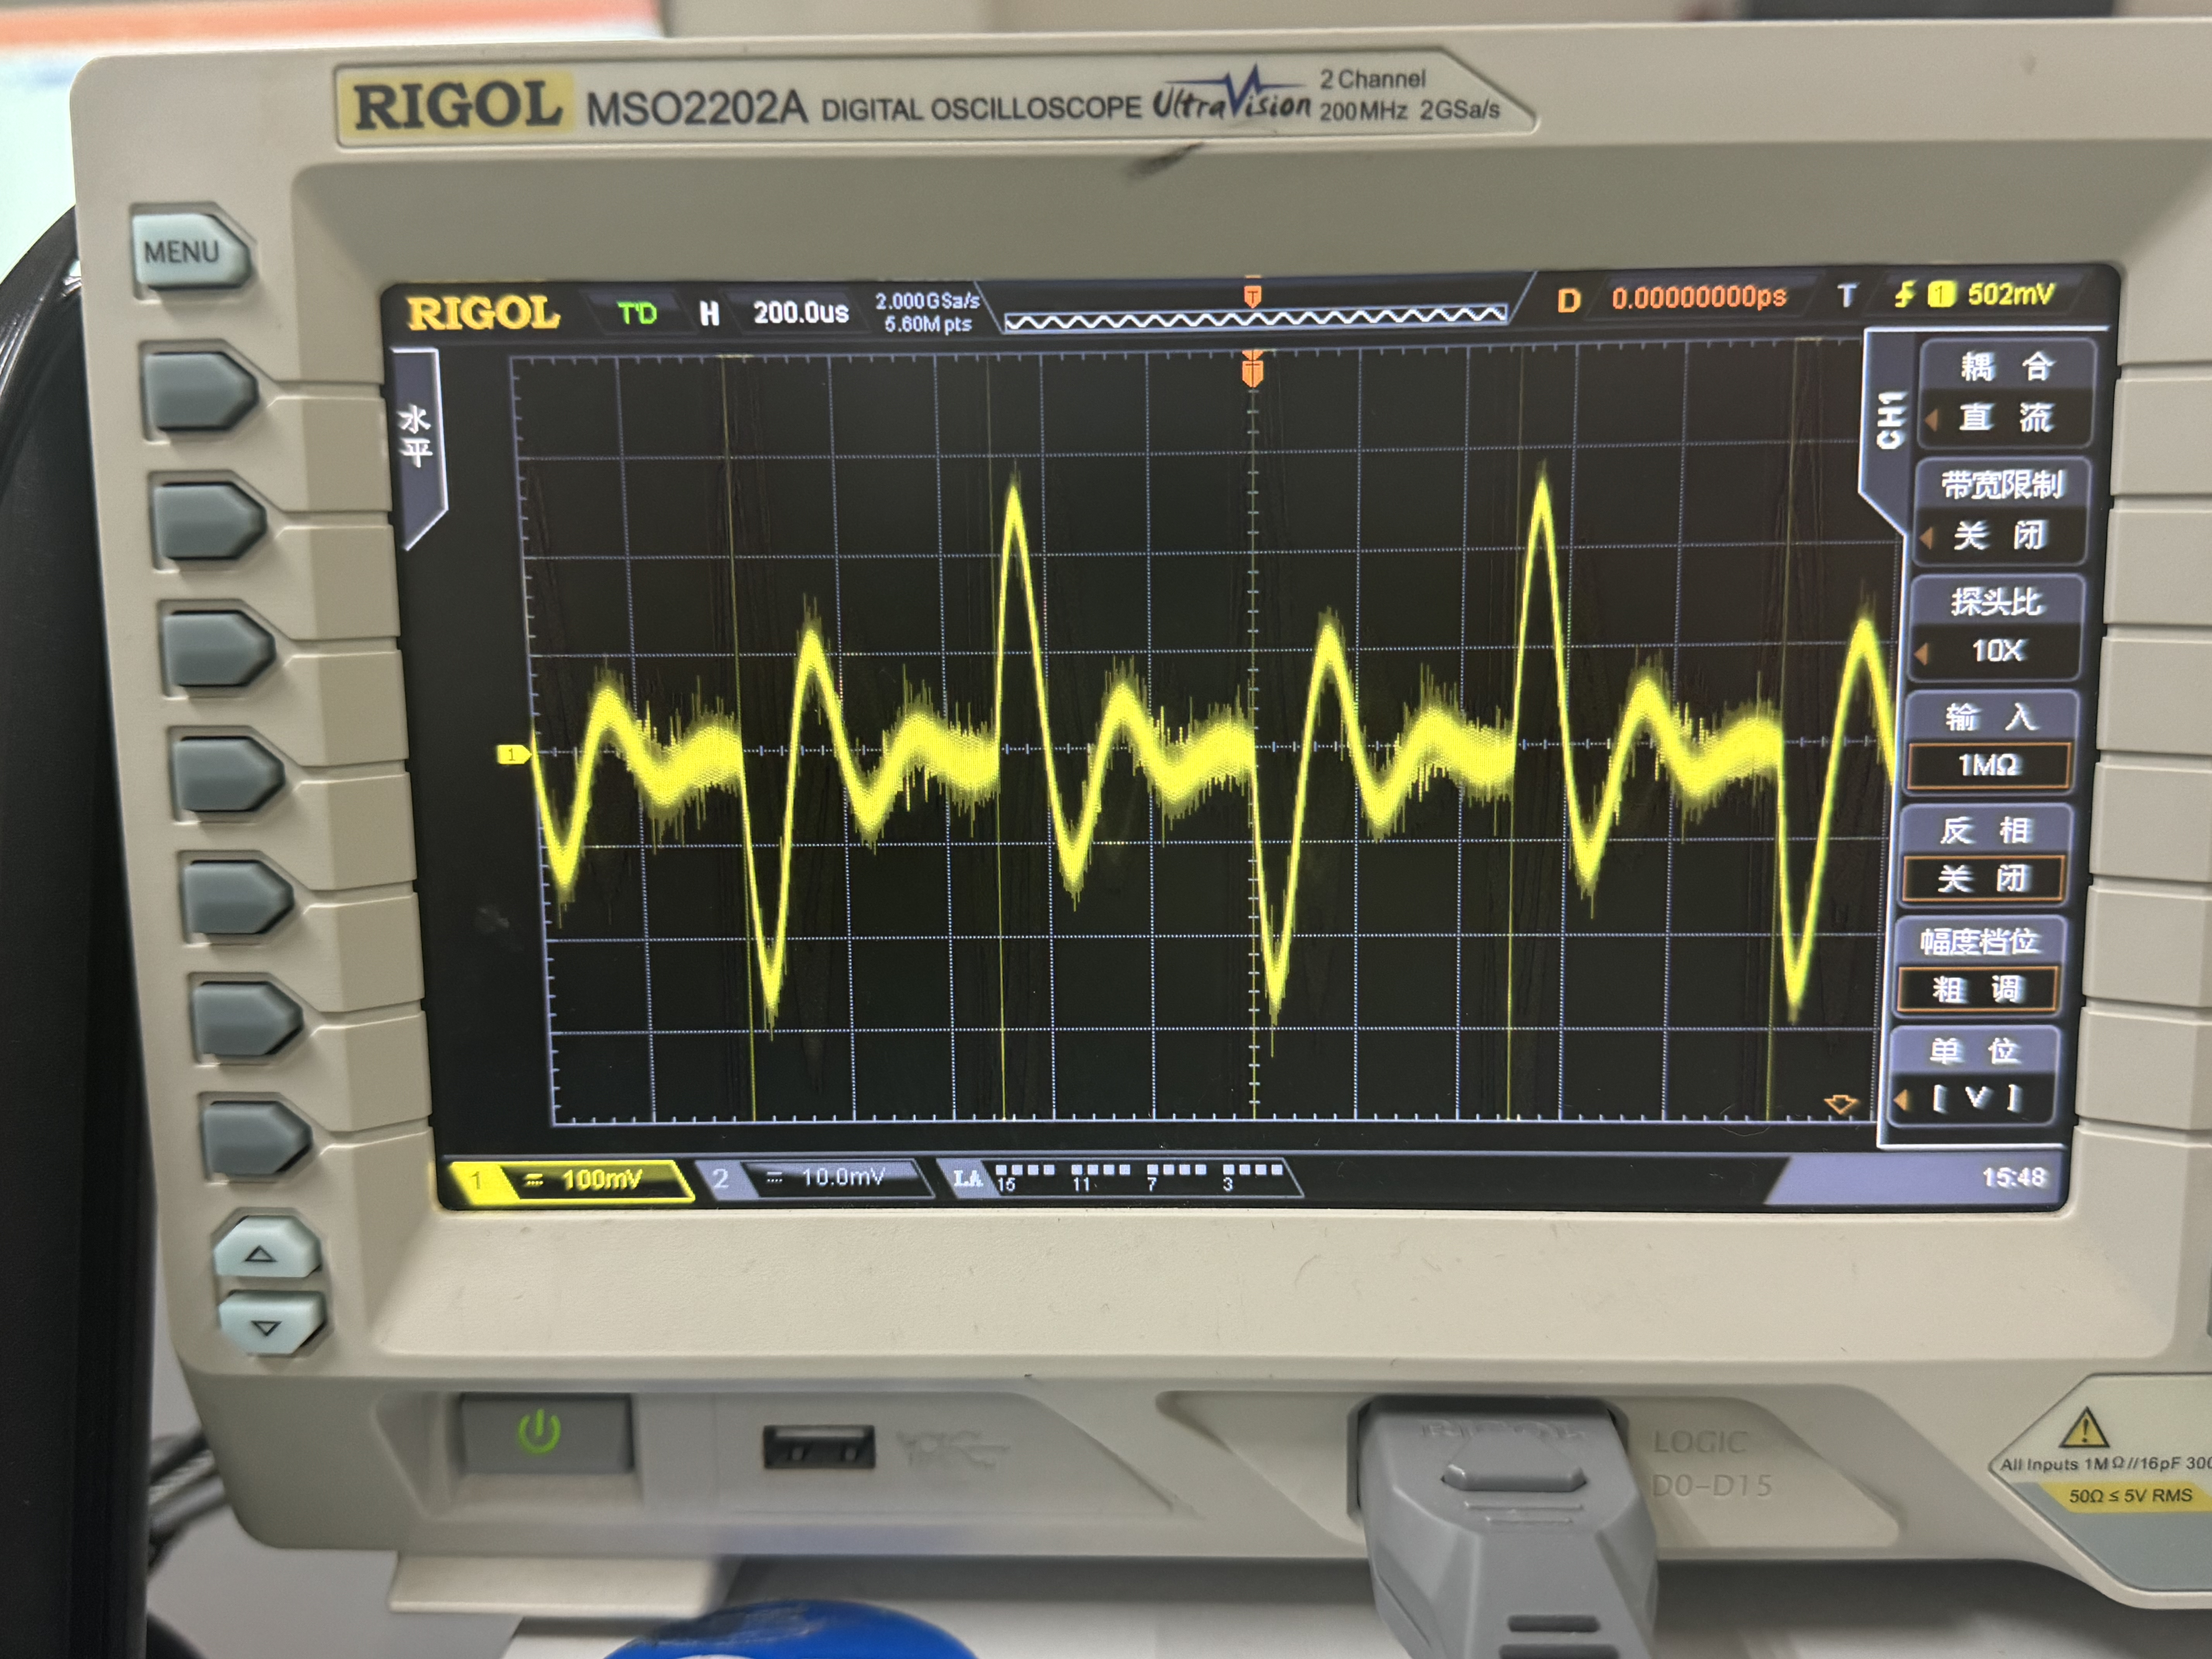
\includegraphics[width=0.35\textwidth]{1Rq.jpg}}
        \caption{欠阻尼实验图像}
    \end{figure}\par
    \clearpage
    \subsection{过阻尼}
    电路参数:$L= \SI{5}{\mH}$,$C= \SI{0.1}{\uF}$,$R=\SI{1000}{\ohm}$
    \begin{figure}[!ht]
        \includegraphics[width=0.71\textwidth]{1g.pdf}
        \caption{过阻尼理论图像}
    \end{figure}
    \begin{figure}[!ht]
        \subfloat[$U_\text{s}$]{\includegraphics[width=0.35\textwidth]{1sg.jpg}}\hspace{6mm}
        \subfloat[$U_\text{C}$]{\includegraphics[width=0.35\textwidth]{1Cg.jpg}}\\
        \subfloat[$U_\text{L}$]{\includegraphics[width=0.35\textwidth]{1Lg.jpg}}\hspace{6mm}
        \subfloat[$U_\text{R}$]{\includegraphics[width=0.35\textwidth]{1Rg.jpg}}
        \caption{过阻尼实验图像}
    \end{figure}\par
    \clearpage
    \subsection{临界阻尼}
    电路参数:$L= \SI{5}{\mH}$,$C= \SI{0.1}{\uF}$,$R=\SI{447}{\ohm}$
    \begin{figure}[!ht]
        \includegraphics[width=0.71\textwidth]{1l.pdf}
        \caption{临界阻尼理论图像}
    \end{figure}
    \begin{figure}[!ht]
        \subfloat[$U_\text{s}$]{\includegraphics[width=0.35\textwidth]{1sl.jpg}}\hspace{6mm}
        \subfloat[$U_\text{C}$]{\includegraphics[width=0.35\textwidth]{1Cl.jpg}}\\
        \subfloat[$U_\text{L}$]{\includegraphics[width=0.35\textwidth]{1Ll.jpg}}\hspace{6mm}
        \subfloat[$U_\text{R}$]{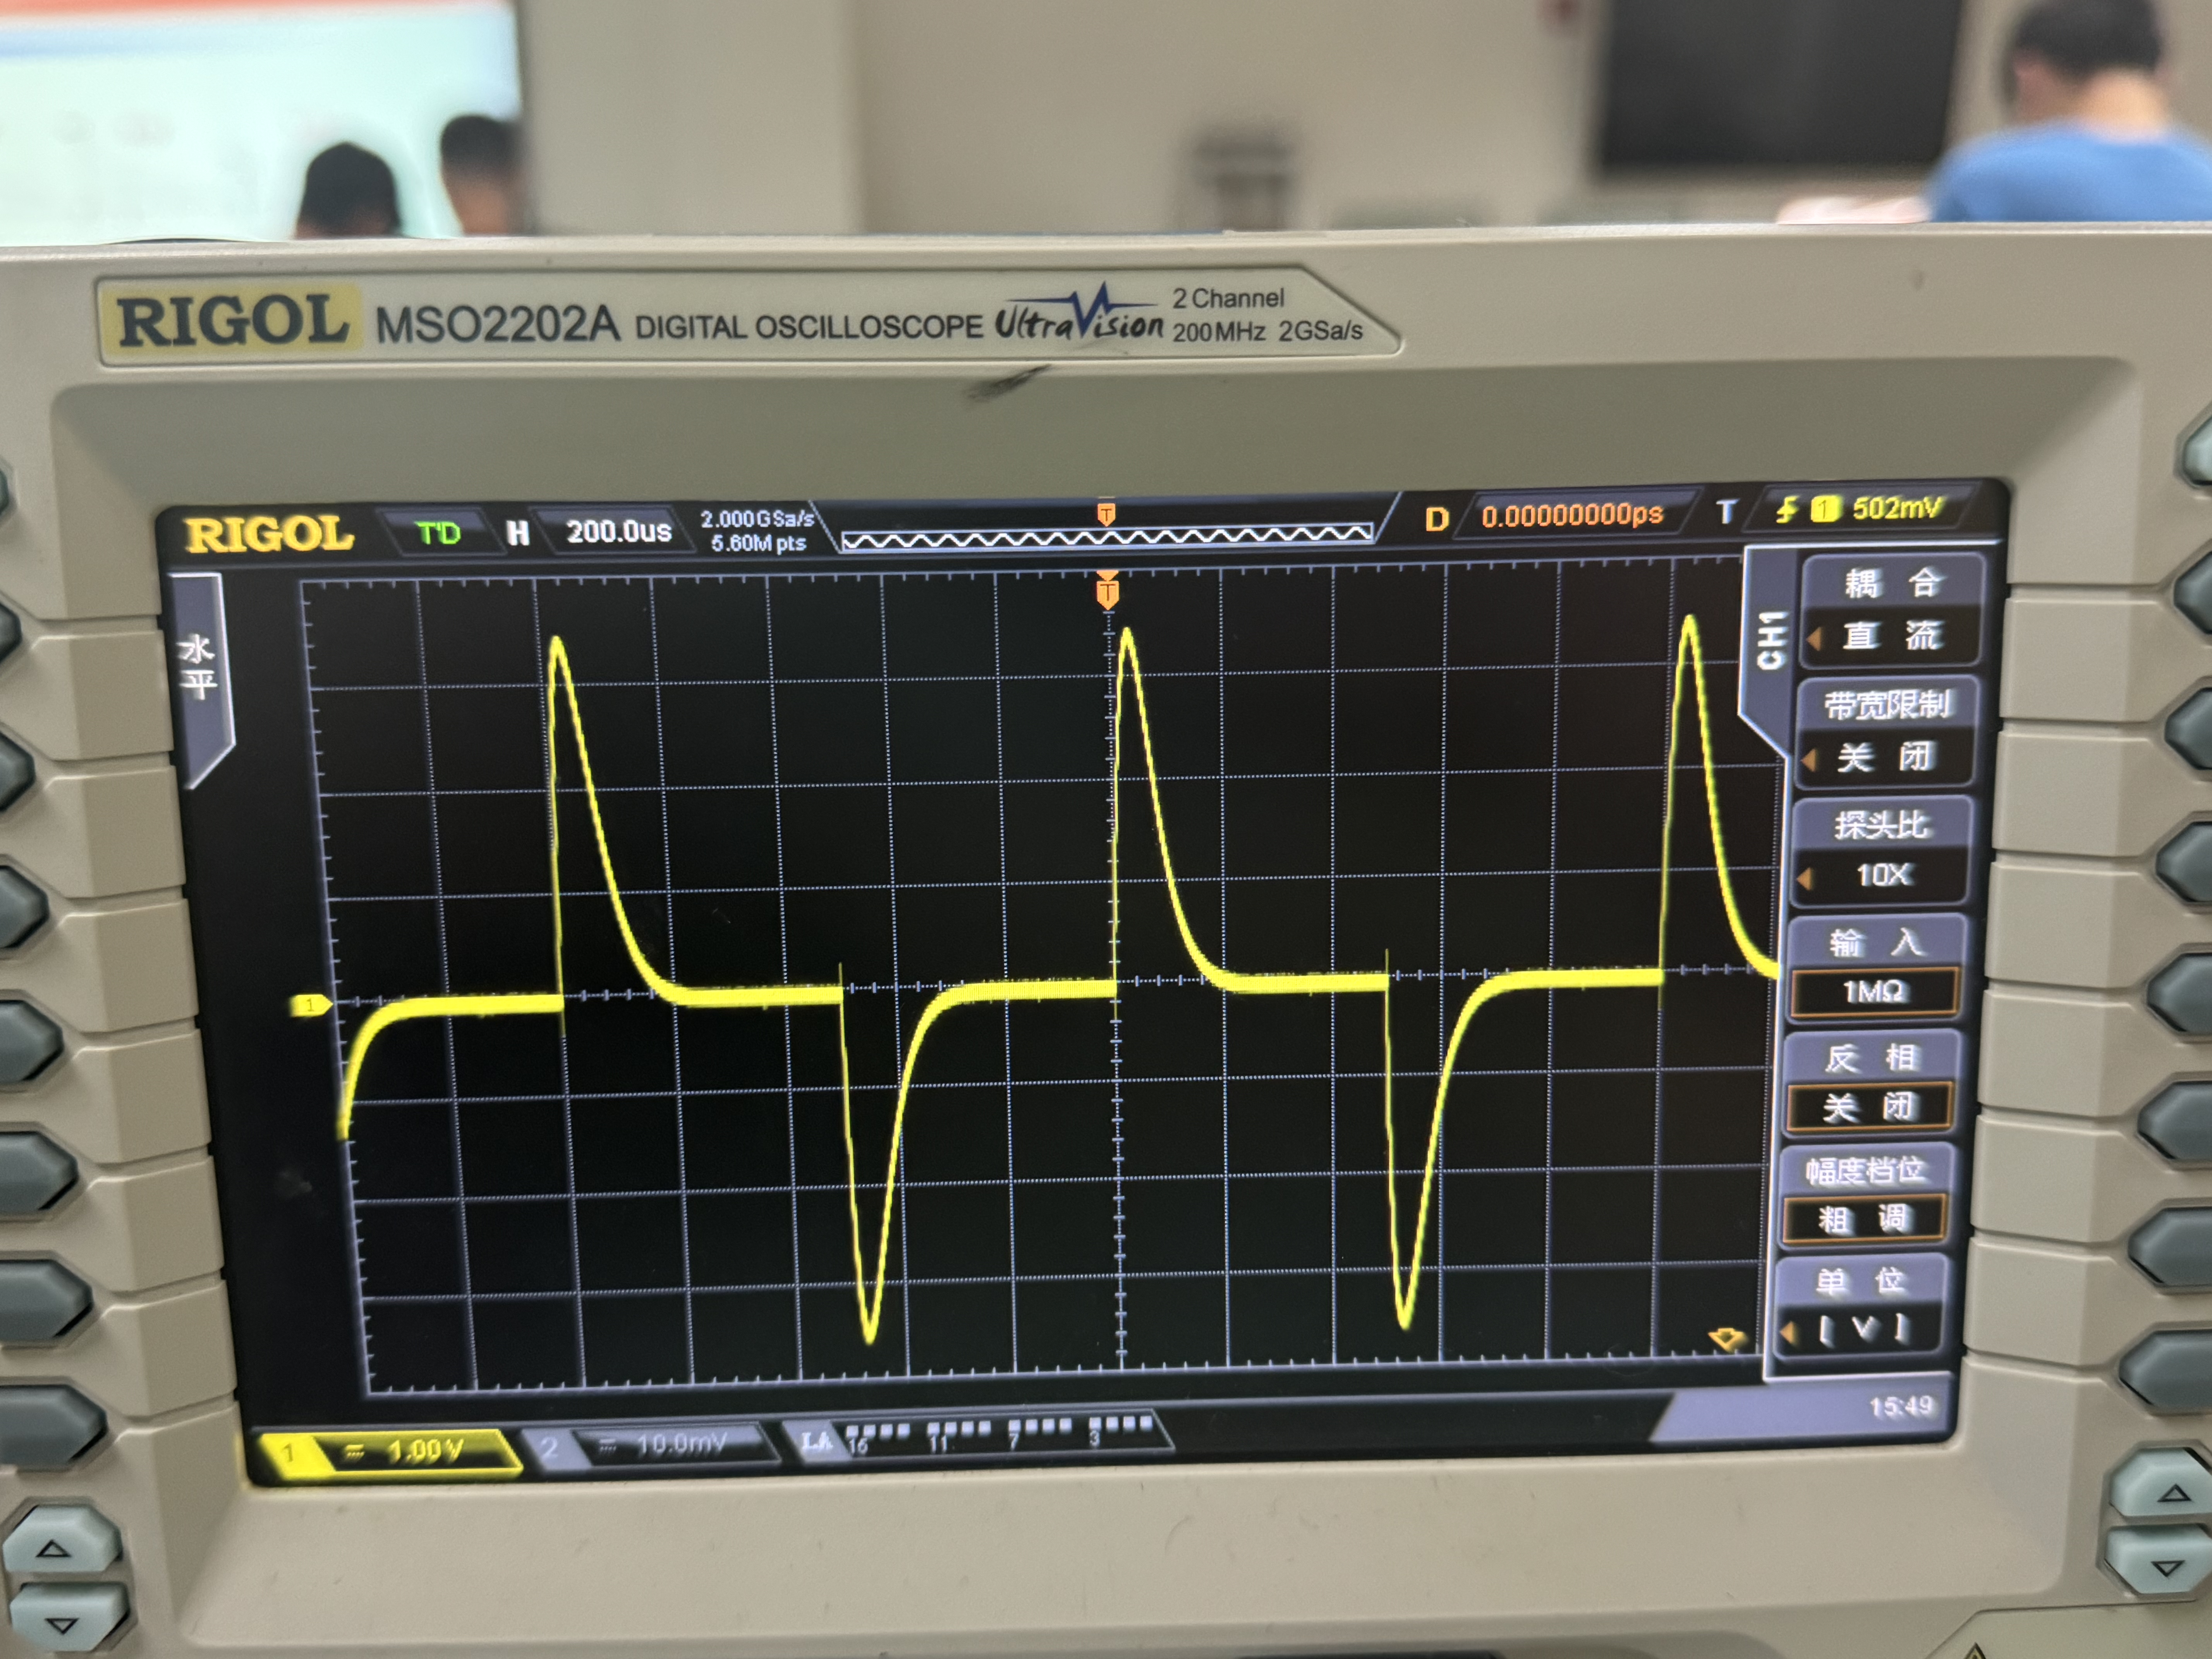
\includegraphics[width=0.35\textwidth]{1Rl.jpg}}
        \caption{临界阻尼实验图像}
    \end{figure}\par
\section{实验分析}
    \subsection{分析}
    由理论计算图与实际测量结果进行比对,发现只有欠阻尼的情况测量较为准确,可能的原因如下:
    \begin{enumerate}
        \item 组件参数误差:
        \begin{itemize}
        \item 电阻、电容和电感的实际值与标称值存在误差。
        \item 温度、老化等因素导致元件参数变化。
        \end{itemize}
        
        \item 电路连接问题:
        \begin{itemize}
        \item 接线错误或松动,导致电路不按照预期工作。
        \item 接触不良或短路,影响电路性能。
        \end{itemize}
        
        \item 示波器设置问题:
        \begin{itemize}
        \item 示波器的时间基准或触发设置不正确。
        \item 示波器探头衰减设置错误(如1X/10X切换)。
        \item 示波器带宽不够,无法捕捉到高频信号成分。
        \end{itemize}
        
        \item 信号源问题:
        \begin{itemize}
        \item 输入信号不稳定或不符合预期波形。
        \item 信号源的频率或幅度设置不正确。
        \end{itemize}
        
        \item 电路模型假设不准确:
        \begin{itemize}
        \item 理论分析时忽略了某些寄生参数,如电感的寄生电阻、电容的漏电阻等。
        \item 实际电路中存在未考虑的非线性元件或其他干扰源。
        \end{itemize}
        
        \item 环境干扰:
        \begin{itemize}
        \item 外部电磁干扰影响测量结果。
        \item 电源噪声或接地不良引入干扰信号。
        \end{itemize}
        
        \item 测量方法不当:
        \begin{itemize}
        \item 示波器探头接地不良,导致测量结果不准确。
        \item 探头加载效应,特别是在高频测量中,探头的输入电容可能影响电路工作状态。
        \end{itemize}
    \end{enumerate}
    \subsection{误差分析}
        \begin{enumerate}
            \item 仪器输出与测量可能产生误差
            \item 线路上的电阻电感电容对结果有一定影响
        \end{enumerate}
\section{思考题}
在实验中,激励源采用方波源而不是手动开关不断进行合、断切换,主要有以下几个原因:
\begin{enumerate}
    \item \textbf{稳定性和精确性}:方波源能够提供稳定且精确的周期性信号,而手动切换无法达到同样的稳定性和精度。手动操作不仅容易出错,还会导致切换时间不一致,影响实验结果的可靠性。
    \item \textbf{频率控制}:方波源可以精确控制切换频率,从而实现对激励信号频率的准确调节。而手动操作难以保持恒定的频率,并且频率范围有限。
    \item \textbf{重复性和可控性}:方波源能够确保每次切换的时间间隔完全一致,这对于许多需要重复测量和精确时间控制的实验来说是至关重要的。手动切换则难以达到这种一致性。
    \item \textbf{自动化和效率}:使用方波源可以实现自动化操作,提高实验效率,减少人为干预和误差。手动切换则需要持续的人工操作,效率低下且容易出错。
\end{enumerate}\par
在实验中,方波源和直流电源的内在联系如下:
\begin{itemize}
    \item \textbf{波形特性}:方波是一种周期性变化的信号,它在一个周期内由两个不同电压值组成(高电平和低电平),在一定时间间隔内不断切换。这种特性与直流电源的开关操作相似,但更为精确和可控。
    \item \textbf{平均电压}:方波的平均电压可以通过调节占空比来控制,占空比是方波周期内高电平时间占总周期时间的比例。当占空比为 50\% 时,方波的平均电压是高电平和低电平的中间值。
    \item \textbf{瞬态响应}:在某些实验中,研究对象对电压变化的瞬态响应很重要。方波源能够提供快速的电压切换,有助于观察和分析瞬态现象,而手动切换无法实现如此快速和准确的变化。
\end{itemize}

综上所述,方波源在提供稳定、精确和可控的周期性信号方面具有显著优势,使其成为实验中激励源的首选。

\section{实验心得}
    本次实验实际观察到了二阶电路的动态过程,对于动态电路又有了更加清晰明确的认知,虽然由于仪器或者操作问题导致实验结果与预期不符。但是在操作过程中,我的实验技能得到了提升,同时对二阶电路的动态过程的理解更加透彻。
\section{原始数据及图形}
    \begin{center}
        \framebox{\rotatebox{-90}{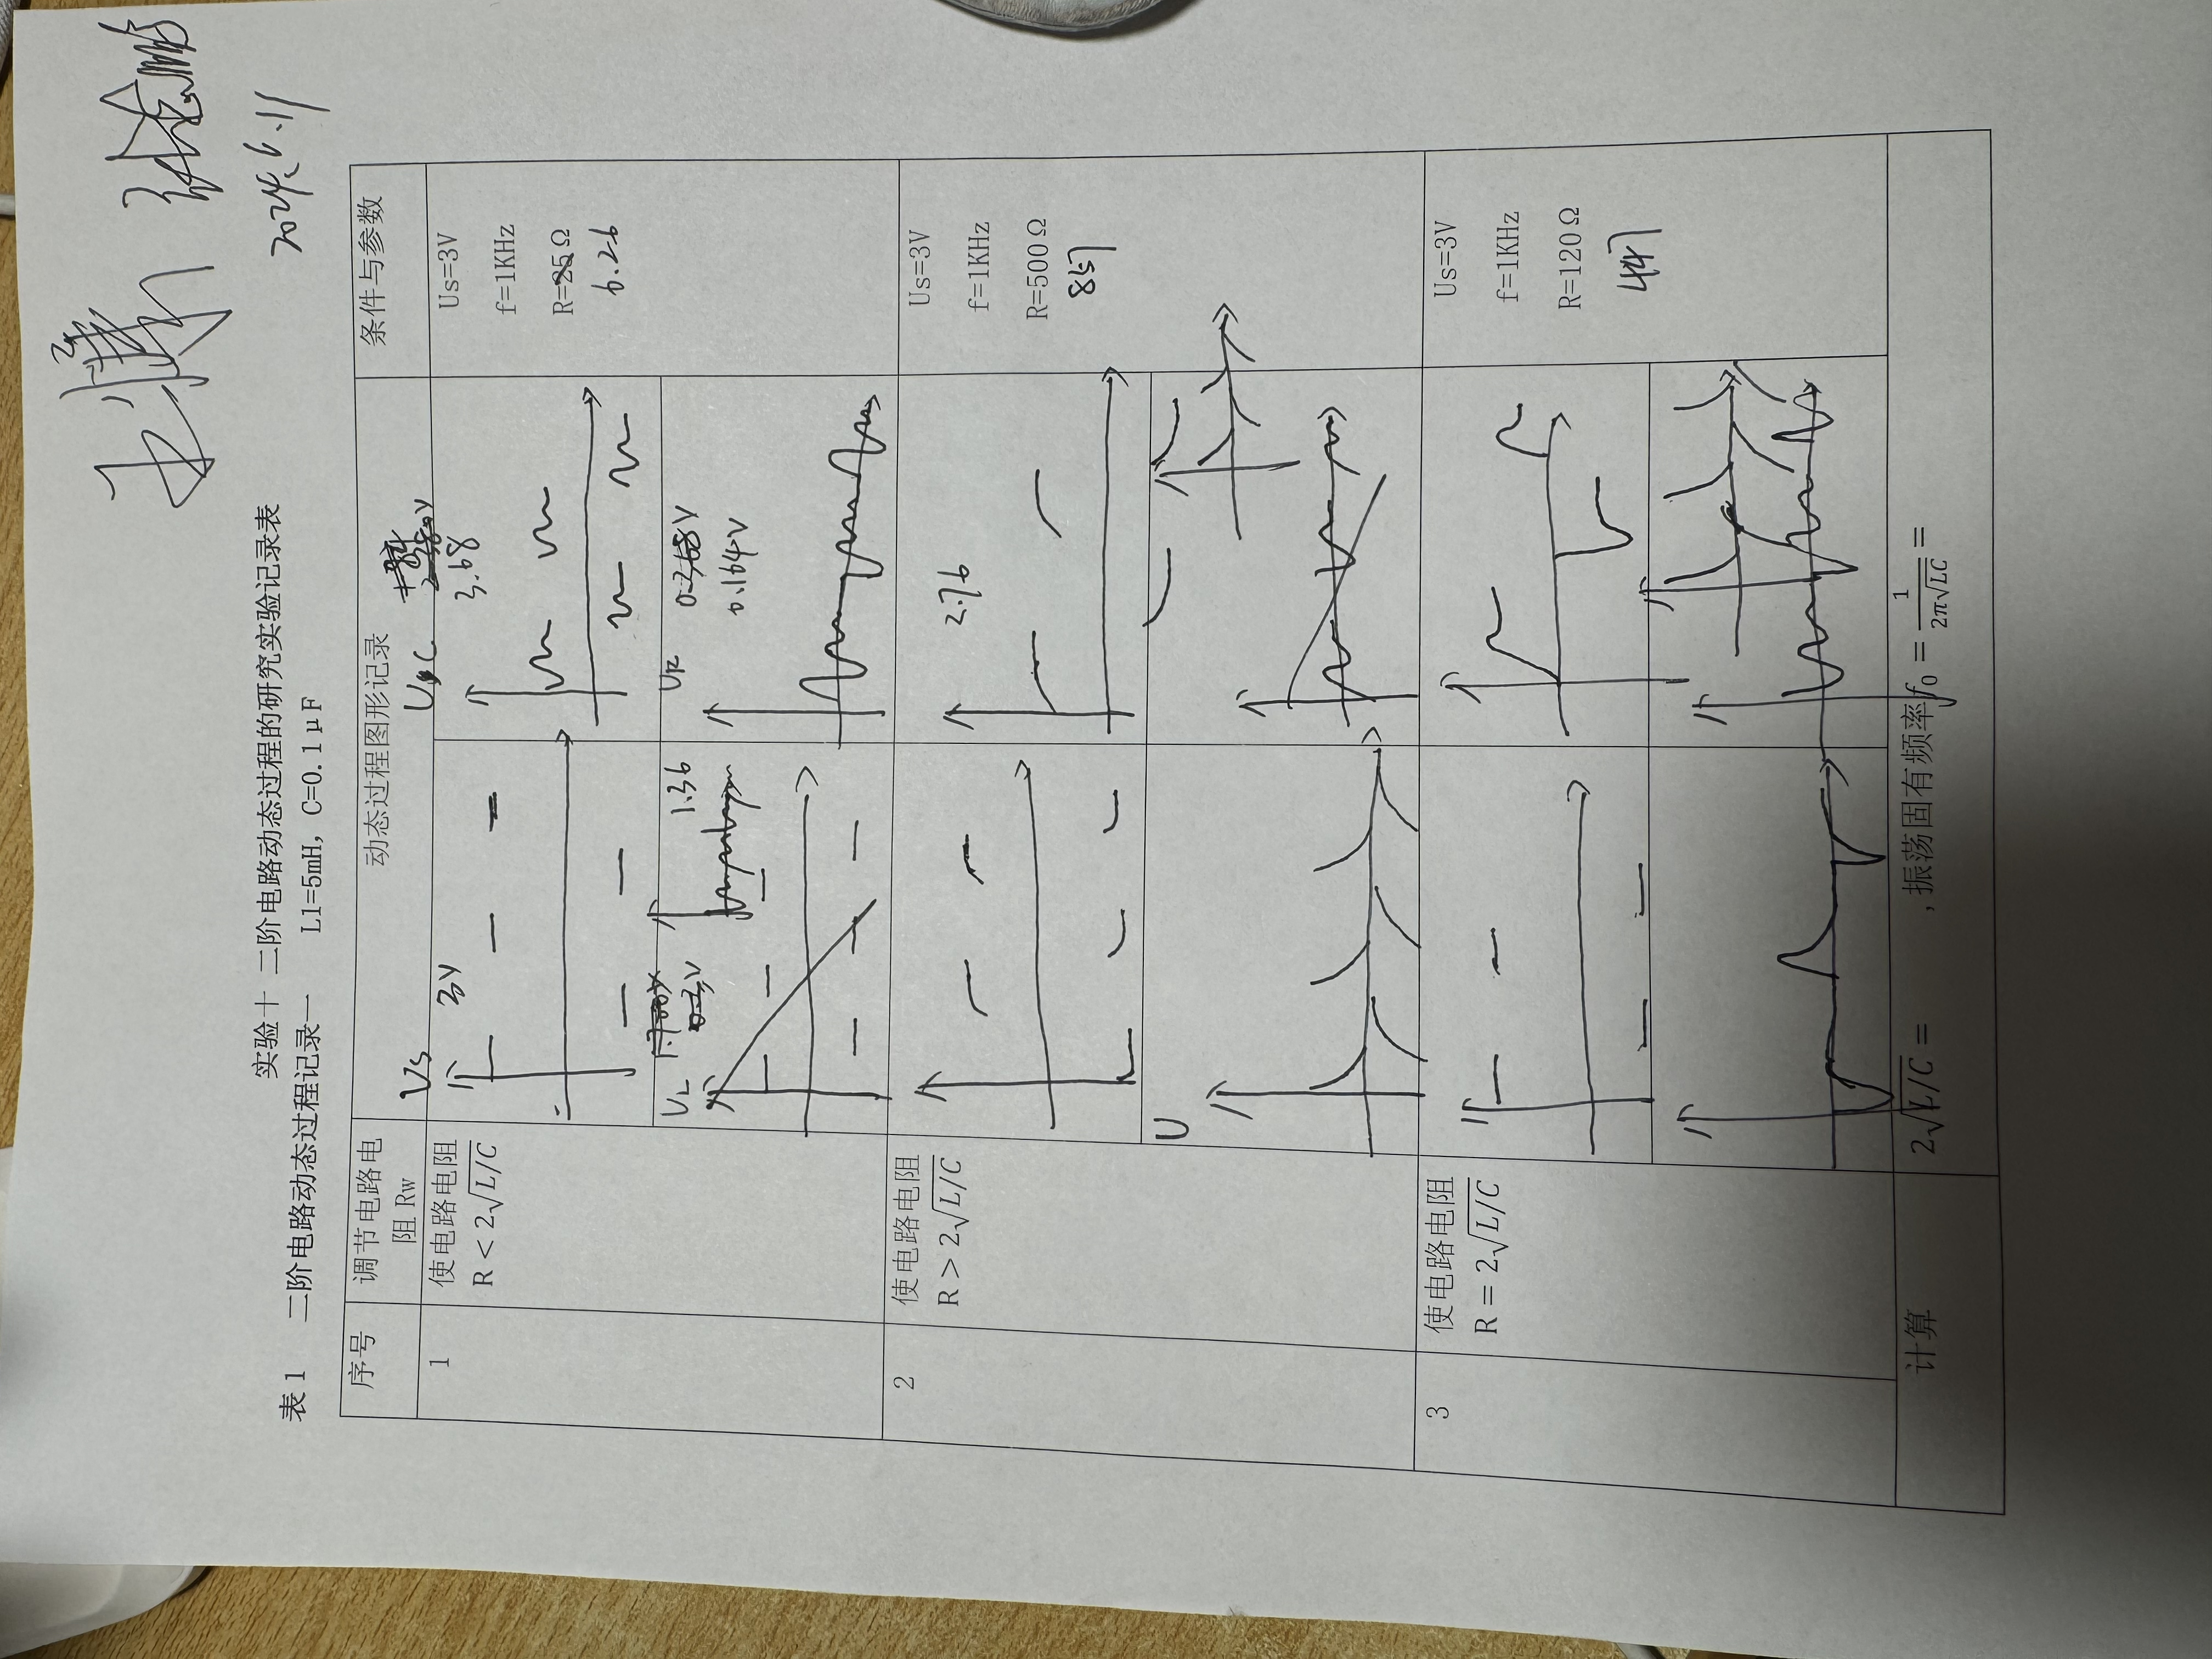
\includegraphics[height=0.8\textwidth]{rawdata.jpg}}}
    \end{center}
    \end{document}